\documentclass[10pt,twocolumn]{article}

% ---- Fonts & encoding ----
\usepackage[T1]{fontenc}
\usepackage[utf8]{inputenc}
\usepackage{amsmath}
\usepackage{newpxtext}   % Palatino-like serif body
\usepackage{newpxmath}
\let\Bbbk\relax          % avoid clash between newpxmath and amssymb
\usepackage{amssymb}
\usepackage{microtype}

% ---- Layout ----
\usepackage[letterpaper,margin=0.75in,columnsep=0.3in]{geometry}
\usepackage{graphicx}
\usepackage{booktabs}
\usepackage{xcolor}
\usepackage{titlesec}
\usepackage{caption}
\usepackage{stfloats}
\usepackage[numbers,sort&compress]{natbib}
\usepackage{listings}
\usepackage[colorlinks=true,linkcolor=black,citecolor=black,urlcolor={blue!55!black}]{hyperref}
\usepackage{xurl}   % allow long URLs to break anywhere
\usepackage{enumitem}

\captionsetup{font=small,labelfont=bf,skip=4pt}
\setlength{\parindent}{1em}
\titlespacing*{\section}{0pt}{1.1ex}{0.6ex}
\titlespacing*{\subsection}{0pt}{0.9ex}{0.4ex}
\titleformat{\section}{\normalfont\large\bfseries}{\thesection}{0.6em}{}
\titleformat{\subsection}{\normalfont\normalsize\bfseries}{\thesubsection}{0.6em}{}

\definecolor{codebg}{gray}{0.96}
\definecolor{kw}{RGB}{140,20,120}
\definecolor{cmt}{RGB}{90,110,90}
\definecolor{str}{RGB}{30,90,160}
\lstset{
  basicstyle=\ttfamily\scriptsize,
  backgroundcolor=\color{codebg},
  keywordstyle=\color{kw}\bfseries,
  commentstyle=\color{cmt}\itshape,
  stringstyle=\color{str},
  language=Python,
  columns=fullflexible,
  breaklines=true,
  showstringspaces=false,
  frame=none,
  xleftmargin=3pt,
  aboveskip=4pt,belowskip=4pt,
  literate={->}{{$\rightarrow$}}2 {→}{{$\rightarrow$}}2 {↔}{{$\leftrightarrow$}}2,
}

\newcommand{\code}[1]{\texttt{\small #1}}
% CommandAGI looped-square mark (the official ⌘ logo path)
\newcommand{\cmdglyph}{\raisebox{-0.13em}{
\includegraphics[height=0.92em]{figures/commandagi-mark.pdf}}}

% ---- Title ----
\title{\vspace{-3.5em}\bfseries Canvas Engineering: Declared Causal Macrostructure\\ for Reverse-Diffusion Latent Dynamics}
\author{\normalsize
  Jacob Valdez\thanks{\href{mailto:jacob@commandagi.com}{\texttt{jacob@commandagi.com}}} \quad \cmdglyph\ CommandAGI\\[0.35em]
  \href{https://commandagi.com/research/canvas-engineering}{\texttt{commandagi.com/research/canvas-engineering}}
}
\date{\normalsize July 2026}

\begin{document}
\maketitle

\vspace{0.4em}

\noindent\textbf{Abstract}\par\vspace{0.4em}
\noindent\small
Prompt engineering structures what a language model \emph{sees}; canvas engineering structures what a diffusion model \emph{thinks in}. The practitioner declares the macrostructure of a diffusion transformer's latent space---which regions carry which modalities, their geometry, temporal update frequencies, loss participation, and, critically, a directed graph of \emph{permitted} block-to-block attention operations---and a compiler lowers that declaration into attention masks, loss weights, and frame mappings. Because reverse diffusion is an iterated denoising map over the whole canvas, a hard connectivity constraint on attention induces an explicit, human-legible causal interaction graph \emph{inside} the generative dynamics, while gradient descent remains free to shape all fine structure within and along the declared edges. This is a neurosymbolic architecture in a precise sense: transparent symbolic macrostructure---a type system, with offsets, signatures, calling conventions, and an ABI---hosted directly within learnable neural mechanics, with no discrete/continuous interface to cross. We give the underlying mathematics---region index sets, the mask construction, the weighted denoising objective, and the reachability semantics that make an absent edge an exact (marginal) independence---and describe the abstraction stack (regions $\rightarrow$ topology $\rightarrow$ typed programs $\rightarrow$ compiled deployment), including the compilation of nested entity schemas into hierarchically coarse-grained canvases. Worked designs span robot manipulation, a compiler-allocated hospital ICU ward with 199 regions, air-traffic control, and a 23-region cortical model that recovers brain-encoder--estimated cortical dynamics at $R^2=0.825$. Early experiments---26 studies, 236 training runs on CogVideoX-2B---include a $1.73\times$ parameter-efficiency result for looped attention ($p<0.001$) and a frozen 350K-parameter configuration that beats 11.7M unfrozen parameters on action prediction. We are explicit that these are small-scale results and read them as calibration rather than narrative. We argue that \emph{declared} latent structure is the production-ready on-ramp to intuition-guided symbolic world modeling: the symbolic model is not synthesized by the network, it is authored by the engineer, and the network learns everything else. Research and code at \href{https://github.com/commandAGI/canvas-engineering}{\texttt{https://github.com/CommandAGI/canvas-engineering}}.\par\normalsize\vspace{0.8em}

\section{Position: two routes to symbolic world models}

Chollet's convergence thesis \cite{chollet2026convergence} holds that much of AI trends toward \emph{intuition-guided symbolic world modeling}: deep-learning-guided program synthesis, because a symbolic model constructs a compact, reusable, highly generalizable representation of a problem from minimal data \cite{chollet2019measure}. This inherits a long argument that connectionism alone under-generalizes and that structure must re-enter the loop \cite{marcus2020nextdecade,garcez2023neurosymbolic}. The thesis names the destination but underdetermines the route.

The dominant proposed route is \textbf{synthesis}: a neural policy emits symbolic programs and is rewarded on their execution. It gains compactness and generalization, but pays for a brittle discrete search and---more corrosively---a hard boundary where continuous representations must be quantized into symbols and back. Canvas engineering takes the dual route, \textbf{declaration}: the human authors the symbolic model up front, not as a program the network emits but as the \emph{interaction topology of latent space itself}, and the neural substrate fills it in. Both routes buy the same asset, a macrostructure acquired without data. Declaration ships today, because it compiles to nothing more exotic than attention masks and loss weights over an off-the-shelf pretrained diffusion transformer \cite{peebles2023dit,yang2024cogvideox}.

The framing is economic. Neurosymbolic methods stay research curiosities as long as the marginal dollar buys more from data than from structure---a corollary of the bitter lesson \cite{sutton2019bitter}. Declared structure changes that calculus precisely where data is expensive: robotics, control, multi-agent coordination, world modeling \cite{ha2018worldmodels,hafner2023dreamerv3,lecun2022path}. Authoring a schema is cheap relative to collecting demonstrations. This paper answers a prior question: \emph{how does one make structure declarable at all} inside a modern generative architecture, and what does it buy empirically?

\paragraph{Contributions.}
(i) \textbf{Canvas engineering}, a declarative interface in which a practitioner specifies latent regions, their connectivity, temporal frequencies, and loss roles, and a compiler lowers the specification to attention masks, loss weights, and frame mappings on a stock pretrained diffusion transformer (\S\ref{sec:mechanism}). (ii) A \textbf{formal account} (\S\ref{sec:math}) showing that absent edges yield exact marginal independence in the generative dynamics---graph reachability as the causal semantics of a masked denoiser. (iii) A \textbf{compiler} from nested typed entity schemas to hierarchically coarse-grained canvases, and a typed process layer for deployment (\S\ref{sec:compile}). (iv) \textbf{Worked designs} across robot manipulation, a 199-region hospital ward, air-traffic control, and a cortical model, plus a structural correspondence to cortical organization. (v) An \textbf{honest empirical read}, summarized from a companion study \cite{valdez2026looped}, that separates what declared structure buys (parameter efficiency, an interface) from what it does not yet (iterative reasoning, free binding).

\begin{figure*}[t]
  \centering
  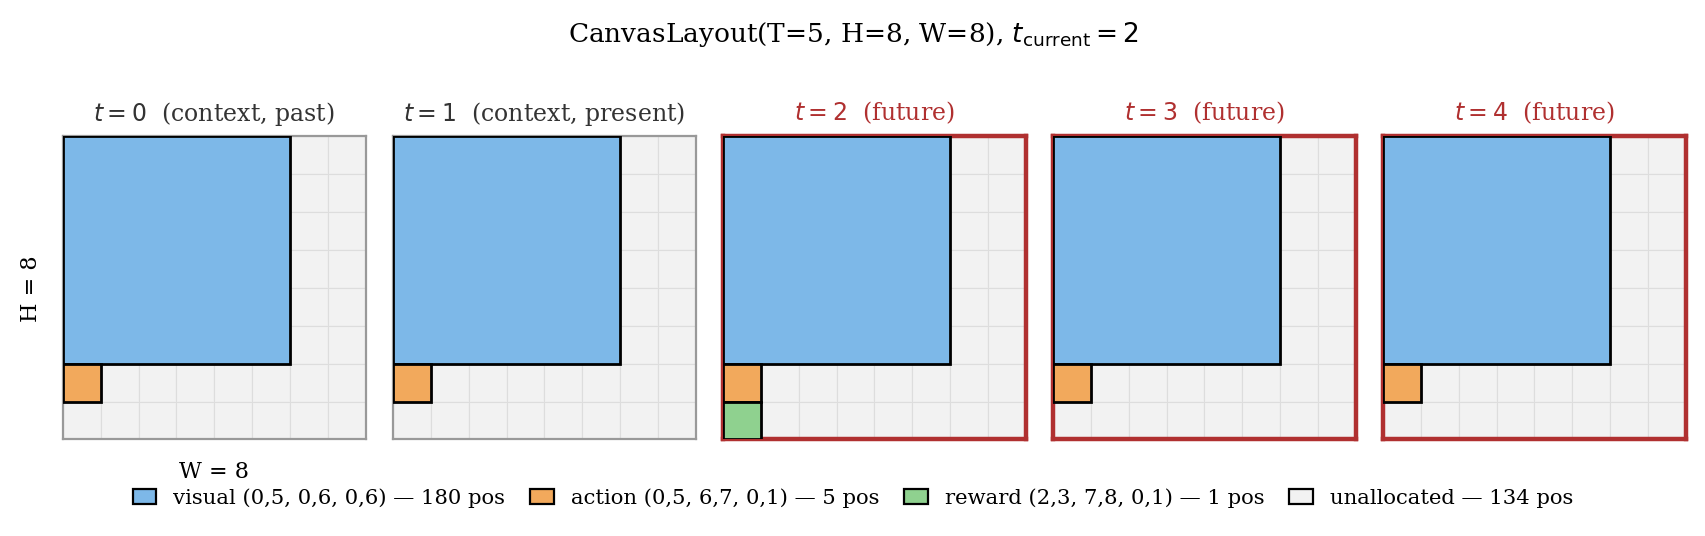
\includegraphics[width=0.94\textwidth]{figures/fig_layout_example.png}
  \caption{The exact layout declared by the code in \S\ref{sec:canvas}, rendered as its five $(H,W)$ time slices. \code{visual} occupies the $6\times6$ block at every frame (180 positions), \code{action} one position per frame (5), and \code{reward} a single position at $t=2$. Frames $t\ge t_{\text{current}}=2$ are future: denoised by reverse diffusion; earlier frames are clamped context. Unallocated positions (gray) carry no loss and no meaning.}
  \label{fig:layouts}
\end{figure*}

\section{Mechanism}
\label{sec:mechanism}

\subsection{The canvas}
\label{sec:canvas}
A \textbf{canvas} is a 3D spatiotemporal grid $(T,H,W)$ of $d$-dimensional latent positions, flattened into the token sequence of a diffusion transformer (DiT). A \code{CanvasLayout} partitions it into named regions (Fig.~\ref{fig:layouts}):

\noindent\begin{minipage}{\linewidth}
\begin{lstlisting}
layout = CanvasLayout(
    T=5, H=8, W=8, d_model=256,
    regions={
        "visual": (0,5, 0,6, 0,6),  # 180 pos - video
        "action": (0,5, 6,7, 0,1),  #   5 pos - actions
        "reward": (2,3, 7,8, 0,1),  #   1 pos - scalar r
    },
    t_current=2,  # t >= 2 is future (diffusion output)
)
\end{lstlisting}
\end{minipage}

Each region carries a \code{RegionSpec}: its bounds; a temporal \code{period} mapping canvas frames to real frames, so a \code{thought} region at \code{period=4} and a \code{perception} region at \code{period=1} coexist on one canvas; \code{is\_output} and \code{loss\_weight}, which make loss participation type-directed codegen---\code{loss\_weight\_mask()} compiles the declaration into a per-position weight tensor; an optional \code{semantic\_type} with a frozen embedding; and a \code{default\_attn} function family. Heterogeneous modalities enter and exit through per-region encoders and decoders; the pretrained video backbone attends over everything. The canvas is thus the omnimodal I/O layer that lets a video model also \emph{do things}---predict actions, read proprioception, estimate reward---rather than only generate pixels.

\subsection{Topology: the causal graph is the attention mask}
A \code{CanvasTopology} is a directed multigraph of discrete cross-attention operations. Each \code{Connection(src, dst)} licenses \code{src} tokens to query \code{dst} keys and values; the \emph{absence} of an edge is a hard prohibition, not a soft prior:

\begin{lstlisting}
CanvasTopology(connections=[
  # action queries visual: obs -> act
  # information flow (diffusion policy)
  Connection(src="action", dst="visual"),
  # action at t queries visual at t-1
  Connection(src="action", dst="visual",
             t_src=0, t_dst=-1),
  # cross-agent coordination
  Connection(src="r1_cam", dst="r2_cam",
             weight=0.5),
])
\end{lstlisting}

Temporal offsets $(t_{\text{src}}, t_{\text{dst}})$ restrict which frame pairs participate---same-frame-only, previous-frame causal, sliding window---and a \code{TemporalFill} mode (\code{HOLD}/\code{DROP}/\code{INTERPOLATE}) resolves cross-frequency queries in real-time space when a \code{period=1} region queries a \code{period=4} one. Convenience constructors---\code{dense} (fully connected), \code{isolated} (block-diagonal), \code{hub\_spoke} (a shared coordinator), \code{causal\_chain} ($A\rightarrow B\rightarrow C$), and \code{causal\_temporal} (same-frame self plus previous-frame cross, no future leakage)---name the standard patterns; a standard transformer \cite{vaswani2017attention} is the degenerate \code{dense} case.

This yields the paper's central claim. Reverse diffusion applies the denoiser to the full canvas at every step \cite{ho2020ddpm,song2021score}, so \emph{which regions can influence which} under iteration is exactly the topology's transitive closure. Declaring the topology therefore declares a causal interaction graph over the generative dynamics---attention-based rather than convolutional, so the graph is over \emph{semantic regions} rather than spatial neighborhoods, and non-Euclidean by construction. Diffusion policy \cite{chi2023diffusion}, observation$\rightarrow$action, is the two-node base case. Multi-agent perceptual diffusion---each agent self-attending over its own observations and actions, coordinating only through declared cross-edges---is the same primitive composed.

What is fixed and what is learned splits cleanly. The engineer fixes \emph{whether} an edge exists, its direction, temporal extent, and function family; gradients---from data or intrinsic losses---determine \emph{what flows} along it and everything within regions. Macro is symbolic, micro is neural, and there is no interface to cross, because the symbolic layer \emph{is} the mask.

\subsection{Core mathematics}
\label{sec:math}
Four small pieces of arithmetic carry the whole construction.

\paragraph{Regions are index sets.} A canvas has $N = T\!\cdot\!H\!\cdot\!W$ positions. A region $r$ with bounds $(t_0,t_1,h_0,h_1,w_0,w_1)$ owns
\[
I_r=\{\,tHW{+}hW{+}w \;:\; t_0{\le}t{<}t_1,\ h_0{\le}h{<}h_1,\ w_0{\le}w{<}w_1\,\},
\]
with regions pairwise disjoint. This is struct-offset arithmetic, nothing more.

\paragraph{The topology compiles to a mask.} Edges $E=\{(r_k{\to}s_k, w_k, \tau_k)\}$ lower to $M\in\mathbb{R}_{\ge0}^{N\times N}$:
\[
M_{ij} \;=\; \max_{k}\; w_k\,\mathbf{1}[i\in I_{r_k}]\,\mathbf{1}[j\in I_{s_k}]\,A_{\tau_k}\!\big(t(i),t(j)\big),
\]
where $A_\tau$ is the temporal alignment predicate: for offsets $(t_{\text{src}},t_{\text{dst}})$, positions align iff $\exists\,\text{ref}: t(i)=\text{ref}+t_{\text{src}},\ t(j)=\text{ref}+t_{\text{dst}}$ (an unset offset is unconstrained). When periods differ, alignment is evaluated in real time $\rho_r(t)=p_r t$, and gaps resolve by fill mode: \code{HOLD} snaps to the most recent past anchor, \code{DROP} yields no edge, \code{INTERPOLATE} distributes weight $\propto 1/d^{\,n}$ over the $n{+}1$ nearest anchors. Execution is per-edge cross-attention, $Y_{I_r} \mathrel{+}= w\,\mathrm{softmax}\!\big(Q_{I_r}K_{I_s}^{\top}/\sqrt{d}\big)V_{I_s}$ (with the edge's \code{fn} substituting the kernel). For a \emph{binary} mask ($w\in\{0,1\}$) this coincides with the monolithic form---adding $\log M$ to dense attention logits with $\log 0=-\infty$; with unequal edge weights the monolithic form is a distinct (approximate) reweighting, since a joint softmax normalizes across edges. The load-bearing case for the causal claim below is the binary mask.

\paragraph{Loss participation is a weight vector.} The declarations compile to $\omega_i=\sum_r \mathbf{1}[i\in I_r]\cdot\code{loss\_weight}_r\cdot\mathbf{1}[\code{is\_output}_r]$, and training minimizes the position-weighted denoising objective
\[
\mathcal{L} \;=\; \mathbb{E}_{x_0,\varepsilon,\sigma}\!\left[\frac{\sum_i \omega_i\,\big\lVert \hat\varepsilon_\theta(x_\sigma)_i-\varepsilon_i\big\rVert^2}{\sum_i \omega_i}\right],
\]
where noise is applied only to output positions at $t\ge t_{\text{current}}$; context positions are clamped to their encodings, i.e.\ conditioning is inpainting-style \cite{ho2020ddpm,song2021score}.

\paragraph{Reachability is the causal statement.} Write the information-flow graph $G$ with an arc $s\to r$ for every connection ($r$ queries $s$, so content moves $s\to r$). One denoiser pass with $L$ attention blocks moves information along paths of length $\le L$ in $G$; $K$ sampling steps compose to a horizon of $KL$. The load-bearing direction is exact and holds by construction, not by regularization: if $G$ has \emph{no} directed path $a\to b$, then $a$ cannot influence $b$'s denoised value, an exact \emph{marginal} independence---the empty-conditioning case of $d$-separation in a graphical model \cite{koller2009pgm,pearl2009causality}. The converse is bounded, not guaranteed: a path of length $\le KL$ makes influence \emph{possible} (the weights may still be zero), while a path longer than the horizon transmits nothing.

\subsection{A type system, literally}
The claim that this is a type system is not decorative (Table~\ref{tab:types}, Fig.~\ref{fig:typesys}). \code{region\_indices()} computes memory offsets; the topology is a calling convention; a serialized \code{CanvasSchema} (layout $+$ topology $+$ metadata, human-readable JSON) is a complete type signature. Two models that share a schema can exchange latent state directly---no tokenization, no re-encoding---because the schema fixes what every position \emph{means}.

\begin{table}[t]
\centering
\small
\caption{The type-system correspondence, item by item.}
\label{tab:types}
\begin{tabular}{@{}p{2.55cm}p{2.25cm}p{2.35cm}@{}}
\toprule
Type concept & Canvas equivalent & Implementation \\
\midrule
Struct field (offset+size) & Region bounds & \code{region\_indices()} \\
Field annotation & period, loss\_weight, sem.\ type & \code{RegionSpec} \\
Pointer / reference & Connection & \code{CanvasTopology} \\
Function signature & Topology + fn & \code{attention\_ops()} \\
Type-directed codegen & Loss mask & \code{loss\_weight\_mask()} \\
ABI compatibility & Schema compat. & \code{compatible\_regions()} \\
Coercion cost & Transfer distance & \code{transfer\_distance()} \\
\bottomrule
\end{tabular}
\end{table}

Across differing schemas, a region can also declare its modality's meaning as a string plus a fixed embedding from a declared model \cite{radford2021clip}, turning modality compatibility from a judgment call into a computable distance (\code{transfer\_distance}): camera and depth should sit far nearer than camera and joint-angles. Whether that distance actually predicts transfer cost is an open calibration, contingent on the representation-stability hypothesis of \S\ref{sec:open}; we make no empirical claim here.

\subsection{Attention function types}
Edges declare \emph{how} information flows, not only \emph{whether}. Seventeen registered function families span dot-product (\code{cross\_}, \code{linear\_}, \code{sigmoid\_attention}), gating (\code{gated}), compression (\code{perceiver} \cite{jaegle2021perceiver}, \code{pooling}), transfer (\code{copy}), state-space (\code{mamba} \cite{gu2023mamba}, \code{rwkv} \cite{peng2023rwkv}), convolution (\code{hyena} \cite{poli2023hyena}), sparse (\code{local\_}, \code{sparse\_attention} \cite{child2019sparse}), and meta (\code{none}, \code{random\_fixed}, \code{mixture}). Resolution order is \code{connection.fn} $\rightarrow$ \code{region.default\_attn} $\rightarrow$ global \code{cross\_attention}. Each choice encodes a theory of the edge---\code{pooling} for a 12-D proprioception summary, \code{perceiver} to bottleneck 864 visual tokens into a thought region, \code{copy} for direct latent relay between agents. The schema declares intent; the executor picks implementation.

\begin{figure}[t]
  \centering
  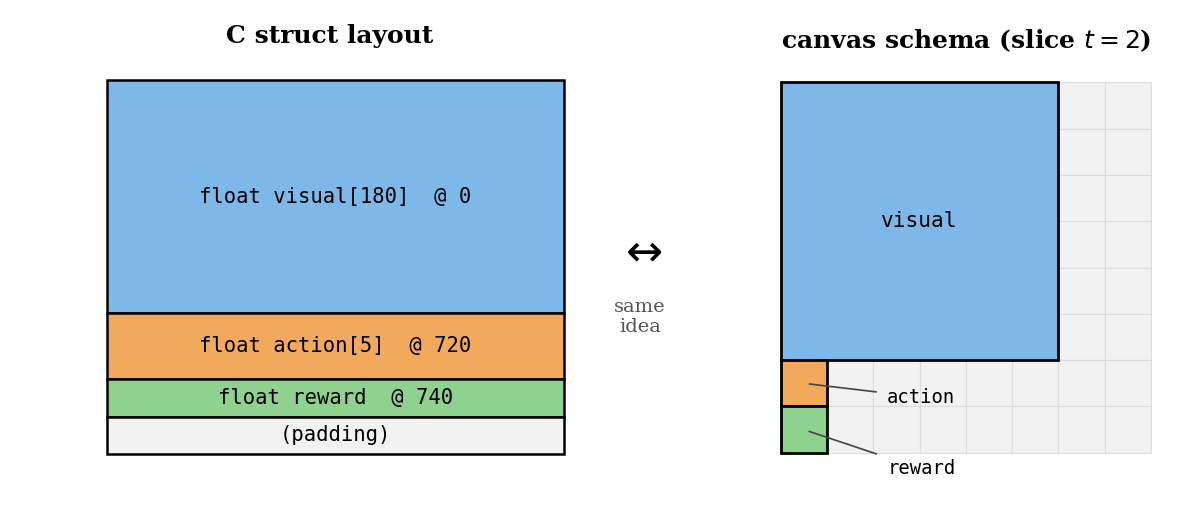
\includegraphics[width=\linewidth]{figures/fig_type_system.png}
  \caption{A C \code{struct} memory layout (left) and a canvas schema (right) are the same object: named fields at computed offsets, with a declared interpretation of every byte / position. The right panel is the $t{=}2$ slice of the layout in Fig.~\ref{fig:layouts}.}
  \label{fig:typesys}
\end{figure}

\section{Compilation: from entity schema to canvas}
\label{sec:compile}

Hand-placing rectangles does not scale, so the compiler accepts typed entity declarations---nested Python dataclasses; a pydantic surface is the same move---and flattens the entity/relationship graph they denote into layout $+$ topology. Every nested type automatically receives a \textbf{coarse-grained field}: a compressed representation that bottlenecks all cross-level attention.

\begin{lstlisting}
@dataclass
class Vehicle:
    __coarse__ = Field(4, 4)   # 4x4 summary
    camera: Field = Field(8, 8)
    plan:   Field = Field(2, 4)
    action: Field = Field(1, 4, loss_weight=2.0)

@dataclass
class Fleet:
    dispatch: Field = Field(4, 4)
    vehicles: list = dc_field(default_factory=list)

bound = compile_schema(
    Fleet(vehicles=[Vehicle() for _ in range(50)]),
    d_model=256)
\end{lstlisting}

Fifty vehicles under dense cross-attention would cost $\mathcal{O}(50^2\!\times\!\text{fields}^2)$ connections; under coarse-graining, each interacts through its $4\times4$ summary---$\mathcal{O}(50\times16)$. Deep nesting chains the bottlenecks: in a world-model schema, the attention path from \code{us.macro.gdp} to \code{cn.macro.inflation} is forced through \code{us.macro} (coarse) $\rightarrow$ \code{us} (coarse) $\rightarrow$ \code{regime} $\rightarrow$ \code{cn} (coarse) $\rightarrow$ \code{cn.macro} (coarse). Each hop compresses, so hierarchical abstraction is not an emergent hope but a topological consequence. In effect the declared schema is a probabilistic graphical model over latent factors \cite{koller2009pgm,pearl2009causality}, compiled into the attention structure of the denoiser rather than into a message-passing runtime.

The \textbf{program layer} (v2) adds process semantics per region: a \emph{family} (observation / state / memory / residual / action), a \emph{carrier} (deterministic / diffusive / filter / memory / residual), a \emph{clock} (periodic or event-triggered, with composable firing rules such as \code{Or(periodic(4), on("err.prediction", gt=0.5))}), and a \emph{compile mode} (runtime / freeze / constant / export). Connection operators are auto-derived from family pairs (observation$\rightarrow$state $=$ ``observe''; state$\rightarrow$action $=$ ``act''); edges can carry triggers (skipped when a predicate over region statistics is false) and learned sigmoid gates. \code{ProgramCompiler} materializes deploy-time semantics: frozen regions get \code{requires\_grad=False}, constants become buffers, and export regions write state dicts to disk. The stack is thus \textbf{entity types $\rightarrow$ canvas schema $\rightarrow$ wired dispatch $\rightarrow$ compiled deployment}, each layer inspectable, serializable, and diffable.

\section{Worked designs}

The abstraction earns its keep on problems whose causal structure is known but whose dynamics are not.

\paragraph{Robot manipulation.}
Vision-heavy, low-latency actions. \code{visual} uses full \code{cross\_attention} for spatial reasoning; \code{proprio} (12-D joints) uses \code{linear\_attention}; \code{visual}$\rightarrow$\code{action} asks which patches matter, while \code{proprio}$\rightarrow$\code{action} is a \code{pooling} summary. This is the configuration behind the empirical results of \S\ref{sec:results}, trained on BridgeData V2 robot video \cite{walke2023bridgev2}.

\paragraph{Multi-agent coordination.}
A vehicle fleet declares per-vehicle self-attention with cross-edges only between neighbors and a shared dispatch hub; an air-traffic conflict-routing schema declares 12 aircraft whose conflict geometry routes through a shared airspace field. Agents never read each other directly---coordination is forced through the shared region we declare between them. The topology \emph{is} the coordination protocol, written as data.

\paragraph{Hospital ICU: causal structure as a type hierarchy.}
The deepest schema in the library (Fig.~\ref{fig:icu}): six patients with organ-level physiology, four nurses with fatigue and workload dynamics, a bureaucratic state (insurance, staffing, bed pressure), and family units. One \code{compile\_schema} call turns that nested instance into 199 regions and 1{,}077 connections on a $26\times26$ canvas---the engineer writes the schema; the compiler does all placement. Each organ system is a nested type with per-field temporal periods that mirror clinical reality (\code{heart\_rate} at \code{period=1}, \code{creatinine} at \code{period=24}, \code{delirium\_risk} at \code{period=12}, \code{loss\_weight=3.0}). A side effect worth stating on its own: the latent tensor becomes \emph{pointable}. One can circle a run of blocks in Fig.~\ref{fig:icu} and say ``that is \code{nurses[1]}''---interpretability not as post-hoc attribution but as a legend for memory, known before training starts. Crucially, the sepsis deterioration pathway---\code{renal.creatinine\_rise} $\rightarrow$ \code{cardiovascular.MAP\_drop} $\rightarrow$ \code{neurological.altered\_consciousness} $\rightarrow$ \code{deterioration\_risk}---is \emph{declared}. A flat model learns the correlation; a canvas model is forced to route through the causal pathway, which is what makes the prediction interpretable and, by hypothesis, robust to distribution shift. Every field has a physiological reason to exist; every edge has a known biological pathway. The type system is not decoration---it is the domain knowledge, made executable.

\paragraph{Cortical world model.}
Declaration taken to its limit: 23 brain regions from the Destrieux atlas \cite{destrieux2010atlas} wired by 42 known cortical pathways (ventral visual stream, the auditory-to-language route, executive control, default mode), across five families---observation (V1, A1, somatosensory), state (association areas), memory (temporal pole), action (motor cortex), and residual (prediction error). The training target is next-timestep cortical activation as \emph{estimated by} Meta's TRIBE v2 brain-encoding model \cite{tribev2} (not measured neural data): from 72 stimuli mapped to 135 regional features, the declared-topology model reaches $R^2 = 0.825$ on next-step prediction while using 19.6\% of possible feature-level connections (3{,}579 of 18{,}225). A separate decoder---4-way category classification from a virtual 20-channel EEG montage sampled from the same TRIBE predictions at 10--20 electrode sites---reaches 68.8\% (linear SVM 59.4\%, chance 25\%). The ablation is instructive: on a low-dimensional (23-scalar) version of the prediction task a small flat MLP wins, and at 135 features a fully dense model matches the cortical one---topology helps convergence and sparsity, not the ceiling. \textbf{Topology is a convergence prior, not a capacity advantage.}

\paragraph{The cortex as existence proof.}
The cortical model is not just another worked example; it is a proof that this fixed-macro / learned-micro decomposition already occurs in a working intelligence. The gross connectivity of the cortex is largely genetically specified---a wiring diagram---while synaptic weights are tuned by plasticity over a lifetime. That is exactly the split canvas engineering makes: the engineer fixes the topology, gradients learn the weights. The correspondence is not merely rhetorical. A cortical connectivity matrix and a canvas attention mask are the \emph{same object}---a source-by-destination matrix, block-diagonal within a functional network, sparse and specific across networks, each entry typed by an operator (see the connectivity-matrix visualization in the repository, whose axes are identical to \S\ref{sec:math}'s $M$). Wiring the declared graph to match known neuroanatomy and recovering the TRIBE-estimated cortical dynamics at $R^2=0.825$---matching a fully dense model at 19.6\% of the connections, and in our runs training several-fold faster because the dispatcher iterates only over the sparse connection set---is a falsifiable structural claim, and its honest reading is the convergence-prior story: the connectome accelerates development without raising the ceiling, just as declared topology accelerates training without adding capacity. One further correspondence is suggestive but we make no mechanistic claim: the cortex clamps sensory input and generates internally when thalamic gating opens, which has the same shape as clamping context regions and denoising output regions---we note the resonance and explicitly do not assert that cortex implements reverse diffusion. The load-bearing point needs no such assertion: whatever the brain is doing, its \emph{structure}---declared macro-topology hosting learned micro-dynamics---is now something an engineer can specify on an arbitrary typed process.

\begin{figure*}[t]
  \centering
  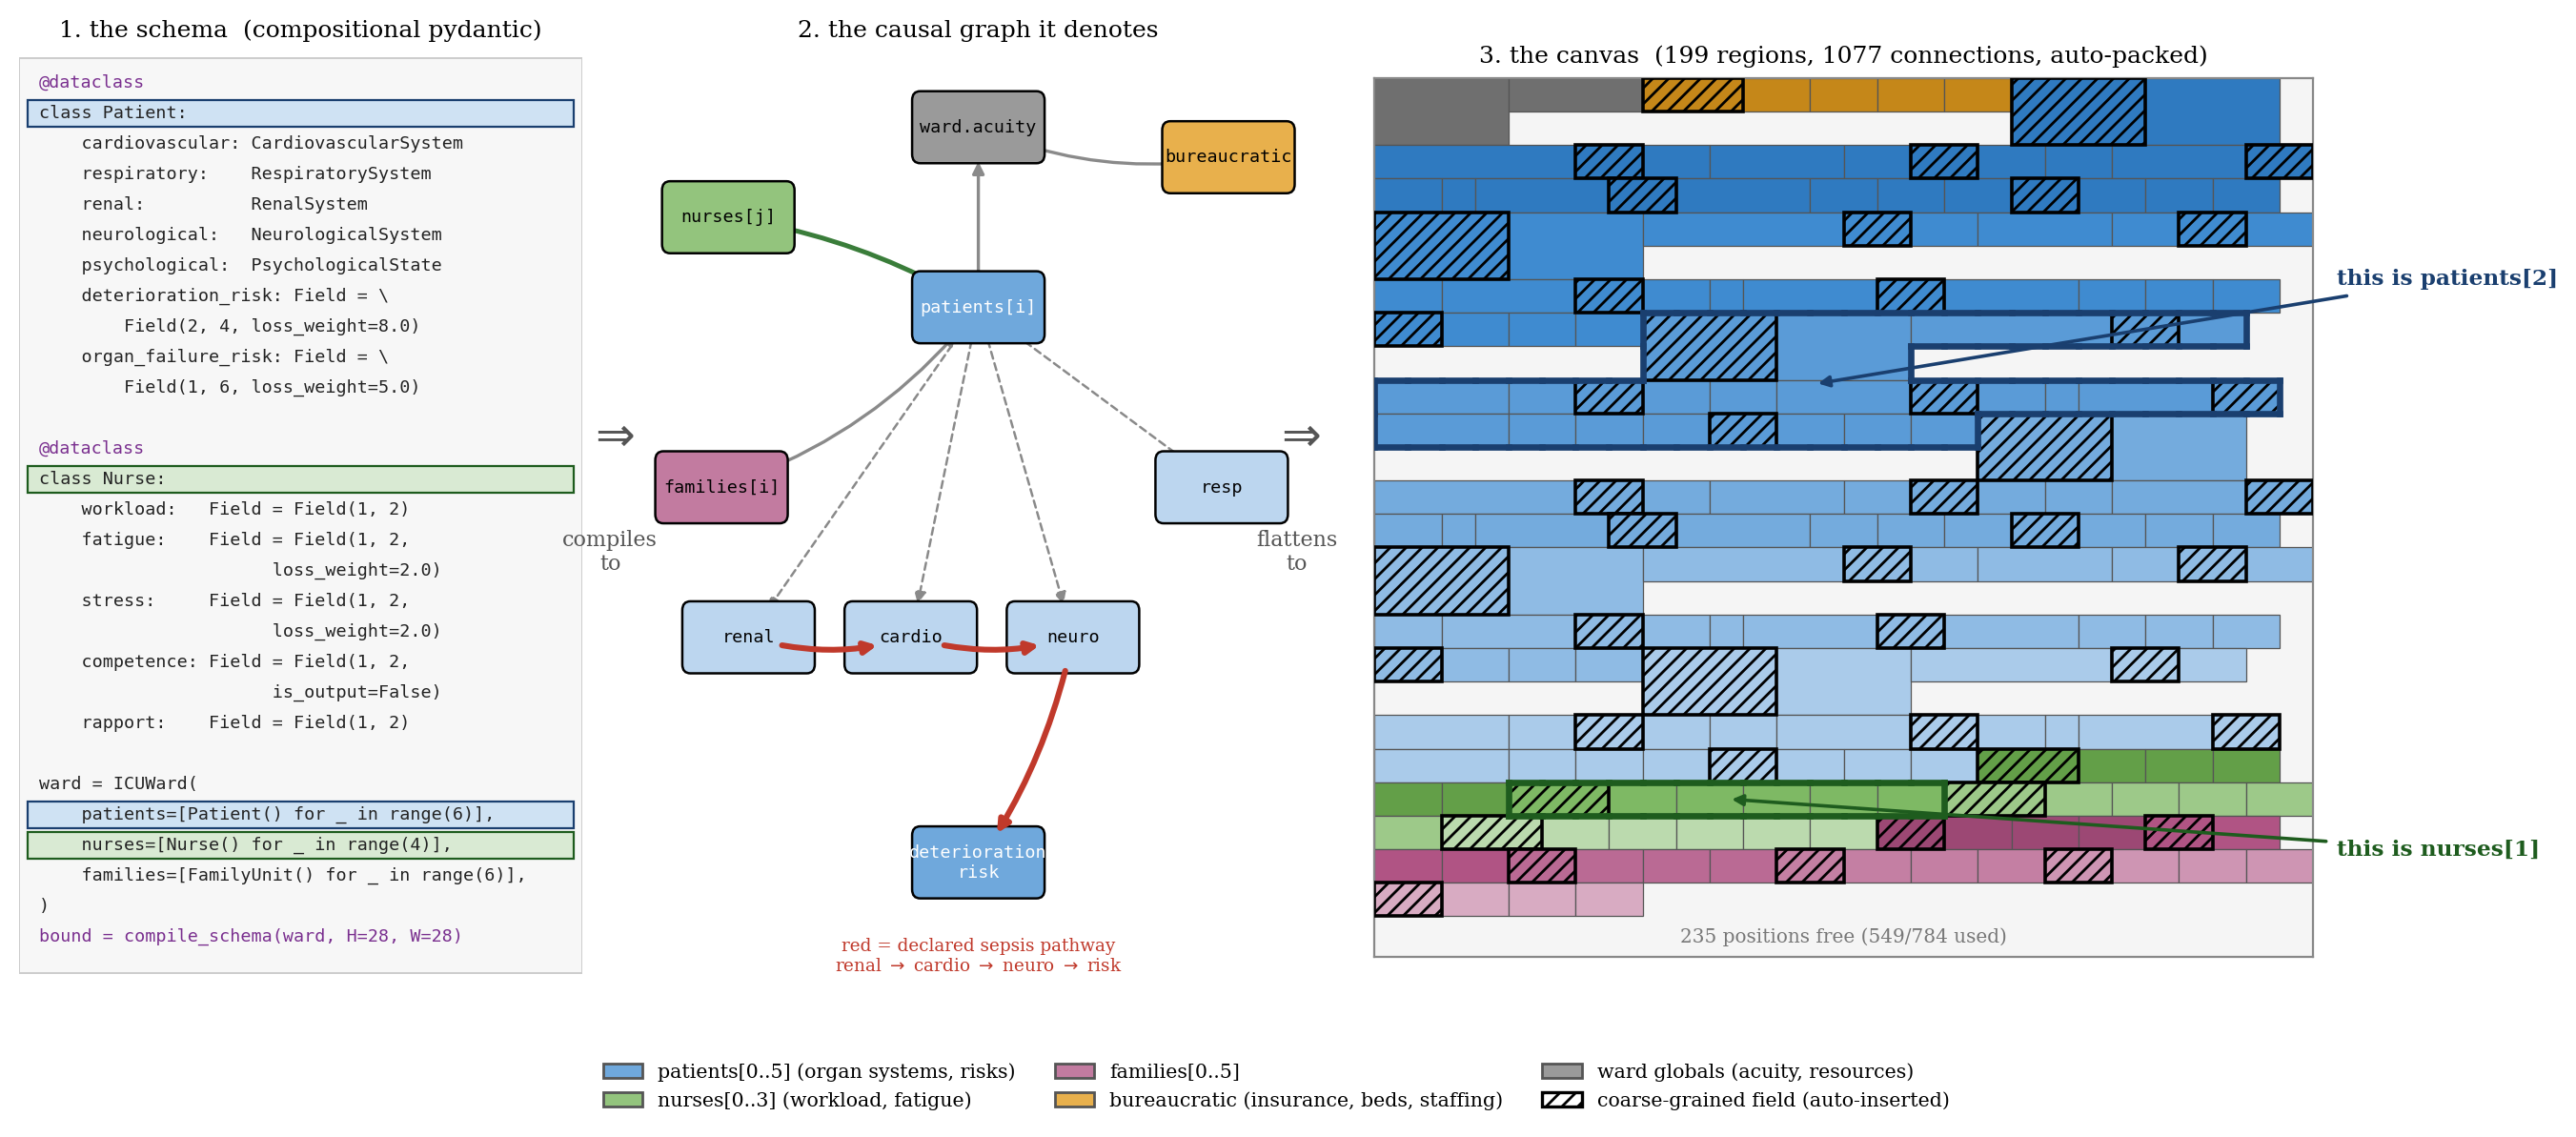
\includegraphics[width=\textwidth]{figures/fig_icu_allocation.png}
  \caption{From schema to canvas, end to end, in three steps. \textbf{1:} the declaration---\code{Patient} and \code{Nurse} types (abridged) and the \code{ICUWard} instance passed to the compiler. \textbf{2:} the causal graph the schema denotes---composition and coordination edges, with the declared sepsis pathway (\code{renal}$\rightarrow$\code{cardio}$\rightarrow$\code{neuro}$\rightarrow$\code{deterioration\_risk}) highlighted. \textbf{3:} the compiler's output---199 typed regions and 1{,}077 connections auto-packed onto a $26\times26$ canvas (68\% utilization), with no manual placement. Hatched blocks are the coarse-grained fields the compiler inserts at every nesting level; all cross-entity attention is forced through them, so the hierarchy of the schema becomes a hierarchy of bottlenecks on the canvas. Because the schema fixes what every position means, the latent tensor is \emph{pointable}: the outlined runs of blocks are, exactly, \code{patients[2]} and \code{nurses[1]}.}
  \label{fig:icu}
\end{figure*}

\section{Empirical record}
\label{sec:results}

The looped-attention results in this section are established, with full protocols, hyperparameters, per-experiment statistical tests, and ablations, in a companion empirical study \cite{valdez2026looped}; we summarize the load-bearing findings and their honest limits here. All results use a CogVideoX-2B backbone \cite{yang2024cogvideox} on BridgeData V2 robot video \cite{walke2023bridgev2}: 26 experiments, 236 training runs.

\paragraph{Looped attention.} Orthogonal to the canvas, looped attention iterates frozen DiT blocks $k$ times with zero-initialized learned iteration embeddings---so at initialization the model is \emph{exactly} the pretrained backbone, with no distribution shift---in the spirit of universal and recurrent transformers \cite{dehghani2019universal,schwarzschild2021thinking}. From a 12-condition grid over loops $\times$ freeze level (Table~\ref{tab:loops}):

\begin{table}[h]
\centering
\small
\caption{Action loss (lower better) across the full $4\times3$ grid (loops $\times$ freeze level; 3 seeds each, 36 runs). Three loops wins at every freeze level; frozen 3-loop (350K trainable params) beats every unfrozen condition (11.7M). Column marginals (mean over loops): 0.110 / 0.120 / 0.108.}
\label{tab:loops}
\begin{tabular}{@{}lccc@{}}
\toprule
 & Frozen & Half & Unfrozen \\
 & (350K) & (3.7M) & (11.7M) \\
\midrule
1 loop  & 0.121 & 0.115 & 0.108 \\
2 loops & 0.140 & 0.119 & 0.112 \\
\textbf{3 loops} & \textbf{0.073} & 0.107 & 0.088 \\
4 loops & 0.104 & 0.137 & 0.124 \\
\bottomrule
\end{tabular}
\end{table}

Recurrence beats depth in parameters: a 3-loop model reaches the loss of a depth-matched baseline carrying $\mathbf{1.73\times}$ its trainable parameters (the estimator and paired test are given in the companion study \cite{valdez2026looped}; $p<0.001$). The freeze main effect is not significant (loop-averaged marginals 0.110 / 0.120 / 0.108 for frozen / half / unfrozen; $p=0.72$); freezing affects video-generation quality instead (an 8--9$\times$ gap on diffusion loss). Loop representations converge toward fixed points (cosine similarity to loop 1: $0.926\rightarrow0.996$; token velocities decay exponentially, action tokens fastest).

\paragraph{Reading the data at the right altitude.} These are 2B-parameter, single-domain, small-data experiments, and we deliberately avoid narratives the data cannot yet carry. Three findings calibrate what the architecture does at this scale, and each one \emph{informs the design} rather than undermining it:
\begin{enumerate}[leftmargin=1.2em,itemsep=1pt,topsep=2pt]
\item \emph{Where looping's benefit comes from.} At this scale the measurable benefit of looped attention is weight-sharing regularization---fixed-point convergence, lower variance, the $1.73\times$ efficiency above---rather than detectable iterative reasoning (three independent nulls). Whether reasoning-like refinement emerges with larger canvases, longer horizons, and more compute is exactly the question the architecture is built to test; we decline to claim it early.
\item \emph{Structure must be declared, not hoped for.} Merely co-locating modalities on a flat, densely-attending canvas did not improve joint prediction---in our runs it degraded it by 19\% ($p<0.0001$). We read this as evidence that binding, like the rest of the structure, has to be declared rather than left to emerge: the capability came from the typed multi-encoder/decoder interface, and co-location alone did not add to it. The natural follow-up---the same canvas with and without declared connectivity---is the next experiment.
\item \emph{Canvas design is forgiving.} Loss is nearly insensitive to token allocation ($\alpha=0.011$: doubling a region's tokens moves loss $0.8\%$). Geometry can therefore serve legibility and engineering convenience without materially taxing accuracy---which is convenient for an interface whose premise is that a human draws the layout.
\end{enumerate}

\paragraph{Reproducibility and scope.} The library, the runnable worked designs, and the schemas in this paper are released open-source (\S Artifacts); the looped-attention experiments---seeds, hyperparameters, per-condition tests, and the full experiment archive---accompany the companion study \cite{valdez2026looped}. Two scope notes. First, the worked designs (the ICU deterioration predictor, air-traffic conflict routing) are \emph{architectural demonstrations} of how causal structure is declared, not clinically or operationally validated systems, and should not be read as such. Second, the cortical result predicts activations produced by a brain-encoding model \cite{tribev2}, not measured neural recordings; extending it to real fMRI/EEG is future work (\S\ref{sec:open}).

\section{Open problems}
\label{sec:open}

\paragraph{Representation stability (the linchpin).} Everything interoperable---schema-mediated latent exchange, transfer-distance calibration, plug-and-play modalities, swap-the-policy-keep-the-perception composition---rests on a platonic-representation-style claim \cite{huh2024platonic}: that identical declared structure induces predictably aligned latent geometry across seeds, datasets, and backbones. Plausible, unproven. The test battery is specified: seed-stability CKA across corresponding regions \cite{kornblith2019cka}; topology$\rightarrow$specialization ablations on fixed data; cross-model grafting cost; and regression of measured transfer cost against semantic-embedding distance.

\paragraph{Binding.} The flat-canvas co-residence penalty (\S\ref{sec:results}) says implicit binding is not free. Whether \emph{declared topology}---the same canvas with authored connectivity---recovers or exceeds independent-model performance is the decisive ablation, and one on which the framework makes a concrete, testable prediction.

\paragraph{Scale.} All evidence is at 2B parameters and robot-video scale. Whether declared macrostructure keeps paying as data grows, or is eventually washed out \cite{sutton2019bitter,kaplan2020scaling}, is open. The bet is asymmetric: schemas cost nothing to author, compile onto pretrained backbones, and can be relaxed edge-by-edge (\code{fn="none"} $\rightarrow$ dense) if they fail to bind.

\paragraph{Learned topology.} Today the graph is authored. The natural continuation---propose-edges / prune-edges under sparsity pressure, with the declared schema as prior rather than hard constraint---would close the loop back to Chollet's synthesis route, with the canvas as the substrate both routes share.

\section{Related work}

Diffusion policy \cite{chi2023diffusion} establishes observation-conditioned action diffusion---the two-node canvas. Unified multimodal DiTs \cite{peebles2023dit,yang2024cogvideox} share one latent sequence but leave structure implicit, to be discovered from surface gradients: the exact move canvas engineering replaces with declaration. Structured-attention mechanisms---sparse patterns \cite{child2019sparse}, Perceiver bottlenecks \cite{jaegle2021perceiver}, state-space and long-convolution mixers \cite{gu2023mamba,peng2023rwkv,poli2023hyena}---supply the executors; the contribution here is not a mechanism but an authorable, compilable, serializable \emph{schema layer} over them. Probabilistic graphical and structural-causal models \cite{koller2009pgm,pearl2009causality} are the ancestors: a canvas topology is a causal graph whose message passing is implemented by a pretrained denoiser's attention rather than by belief propagation. World models \cite{ha2018worldmodels,hafner2023dreamerv3,lecun2022path} motivate the target application. Looped and universal transformers \cite{dehghani2019universal,schwarzschild2021thinking} study recurrence as adaptive compute; at the scales we have tested, its practical value on frozen video backbones is weight-sharing regularization.

\section{Conclusion}

The neurosymbolic program stalls in production because it usually demands a new runtime at the neural/symbolic boundary. Canvas engineering dissolves the boundary instead: the symbolic artifact is a schema---a type system for latent computation---and its execution is masked attention inside a stock diffusion transformer. You declare the causal macrostructure of thought; SGD fills in the rest. The empirical record is early and we present it at face value: $1.73\times$ parameter efficiency, a 350K-parameter configuration that beats 11.7M, and calibration results that tell us where structure must be declared rather than hoped for. The decisive experiments---declared topology versus flat co-residence, representation stability across seeds and backbones, behavior at scale---are specified and awaiting compute, and we would rather run them than speculate ahead of them. What stands regardless is the abstraction. Once latent structure is \emph{declarable}, it is versionable, diffable, compilable, and shareable---and structure you can ship is the only structure that will ever out-compete paying for more data.

\vspace{0.4em}
\noindent\small\textbf{Artifacts.} \href{https://pypi.org/project/canvas-engineering/}{\code{pip install canvas-engineering}} (Apache 2.0), published under \href{https://commandagi.com}{CommandAGI}. Code: \href{https://github.com/commandAGI/canvas-engineering}{\texttt{github.com/commandAGI/canvas-engineering}}; documentation, runnable examples, and design notes: \href{https://commandagi.com/research/canvas-engineering}{\texttt{commandagi.com/research/canvas-engineering}}. Full experiment archive and the companion empirical paper (``Looped Attention in Video Diffusion Transformers: 26 Experiments on What Works, What Doesn't, and Why'') at \href{https://github.com/JacobFV/recursive-omnimodal-video-action-model}{\texttt{github.com/JacobFV/recursive-omnimodal-video-action-model}}.

{\small
\bibliographystyle{unsrtnat}
\bibliography{references}
}

\end{document}
